\begin{figure}[H]
	\begin{center}
		  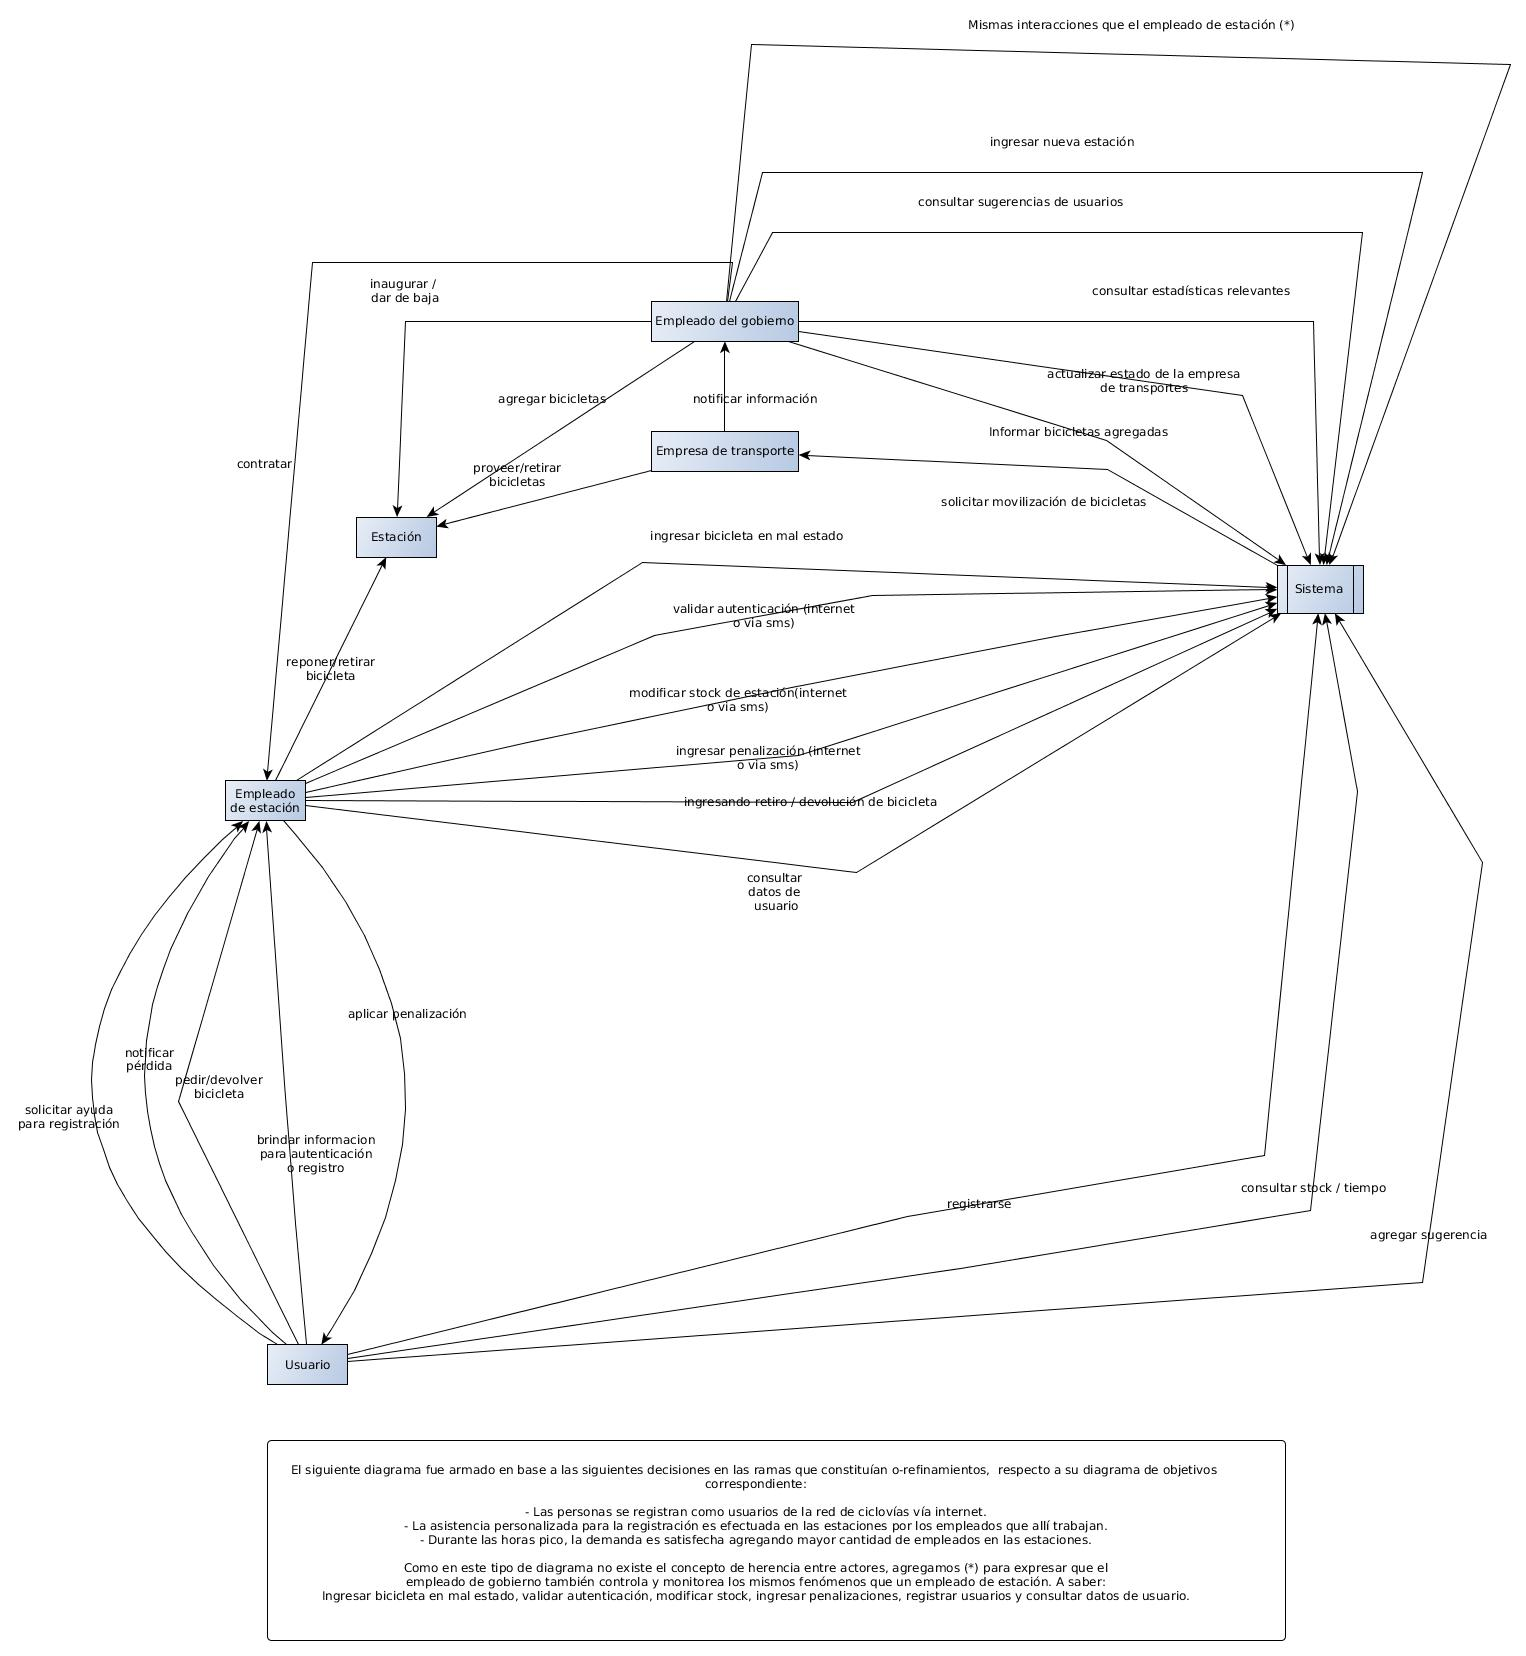
\includegraphics[scale=0.35]{diagrama_contexto.jpg}
		  \caption{Diagrama de contexto}
		  \label{fig:contra1}
	\end{center}
\end{figure}

Los eventos relacionados con nuestra red de ciclovías son controlados y monitoreados por distintos agentes. Cada uno de ellos cumple una función única dentro de la red.
Los usuarios comienzan registrándose por internet brindando los datos requeridos. Entre ellos se destacan principalmente el número de DNI y el nombre completo, ya que ambos serán utilizados
para validar la identidad cada vez que quieran hacer uso de la red. 

En el caso de tener dificultades para completar este proceso pueden acercarse a una de las estaciones y solicitar ayuda a uno de los empleados.
Siempre que un usuario quiera acercarse a una estacion para retirar una bicicleta tiene la opción de consultar previamente la disponibilidad de stock. En caso de estar agotado, el sistema informará el tiempo
estimado en el cual se repondrá.

A la hora de alquilar una bicicleta el usuario le comunica su nombre completo y su DNI al empleado. El empleado de estación valida con el sistema la información recibida y posteriormente le comunica
los resultados. Si existe un problema de autenticación el empleado le solicita que se registre nuevamente. De lo contrario el usuario será autenticado con éxito. Posteriormente, el empleado chequea 
su estado, en donde busca existencia de alquileres pendientes o penalizaciones que no han sido cumplidas. En el caso de no encontrar anormalidades, el usuario
recibe una bicicleta para ser utilizada, la cual deberá devolver en un lapso de tiempo menor a 1 hora.

Si el usuario pierde la bicicleta, o la misma sufre un desperfecto importante durante su uso debe notificarlo en alguna de las estaciones. Ambos hechos serán sancionados e ingresados al sistema
por parte del empleado. Por el contrario, si el usuario devuelve la bicicleta en tiempo y forma, el alquiler finaliza y el usuario podrá retirar nuevamente otra bicicleta sin ningún inconveniente.

Los usuarios pueden dejar sugerencias y comentarios en el sistema, que serán tenidas en cuenta por los empleados del gobierno de Mar Chiquita.

El empleado de estación es el encargado de validar la autenticación de los usuarios, otorgar y recibir las bicicletas, consultar el estado de los usuarios, aplicar las penalizaciones (negando la posibilidad
de que efectúen alquileres), colaborar con la empresa de transportes en la movilización (cargando y descargando las
bicicis) e ingresar los datos al sistema. Entre los datos que puede registrar se destacan: la modificación del stock de bicis, el inicio o cierre de un alquiler, 
el ingreso de una penalización, el ingreso de una bicicleta en mal estado o de un extravío.

El stock en una estación se modifica cuando se retiran bicicletas para satisfacer un pedido, o cuando se reciben bicicletas debido a un pedido. En ambos casos, es el empleado de estación quien actualiza esta información en el sistema.

El stock disponible en cada estación a cada hora, y las movilizaciones entre estaciones son manejadas en su totalidad por parte del sistema mediante un algoritmo
, ya que este último es el que dispone de toda la información necesaria para calcular la mejor distribución (considerando que la demanda es mayor en las estaciones del centro en el horario pico). 
Los empleados no pueden realizar pedidos a la empresa de transporte ya que es responsabilidad del sistema, aún cuando la estación agota su stock.

El sistema provee una api que permite cargar y enviar los datos a través de sms's enviados por los empleados en los casos en los que se pierde la conexión a internet en sus respectivas estaciones. 

Las bicicletas están distribuídas en las estaciones. Periódicamente nuevas bicicletas son agregadas por parte de los funcionarios del gobierno para reponer las que se han roto o han sido extraviadas.
Simultáneamente las nuevas bicicletas son ingresadas al sistema, pasando a formar parte de la red.

La empresa de transporte responde a los pedidos que recibe por parte del sistema. En el caso de que surja un inconveniente (por ejemplo, menor disponibilidad de camiones para traslados o imposibilidad de realizar
determinados pedidos), la misma le informa a uno de los empleados del gobierno y este último carga dicha información en el sistema. 
 
El sistema calcula y actualiza constantemente estadísticas recolectadas a partir de los alquileres, las penalizaciones, el stock en cada momento del día, etc. Dicha información es utilizada para mejorar
el algoritmo de predicción y distribución, y al mismo tiempo puede ser consultada por los empleados del gobierno.

Estos últimos pueden realizar cualquier actividad asociada a un empleado de estación (no así a la inversa). (Consultar datos de usuarios, cargar y cerrar alquileres, etc.). A su vez, son responsables
de contratar y dar de baja a empleados (tanto de gobierno como de estaciones), inaugurar y dar de baja estaciones, consultar las sugerencias y validar los registros. 
Este último punto es de fundamental importancia, ya que los usuarios no pueden comenzar a retirar bicicletas si sus registros no han sido validados. 